\chapter{Doing Laundry: Folding Score Examples}\label{app:score-folding}

\section*{Definition}
Folding a t-shirt means taking a flat, spread-out shirt and moving one part of it on top of another along a straight line, making the shirt smaller in at least one direction.
A fold counts as successful if the folded part lies flat on top (not bunched or raised), its edges line up reasonably well with the edges underneath, and no accidental creases appear outside the intended fold line.
A full folding task is a series of these folds done in order, with the end goal of ending up with a neat, roughly rectangular flat shape.

\section*{Folding Quality Evaluation}
\textbf{Folding quality is evaluated by neatness and whether the cloth is flattened and stacked.}

Penalties for human assistance during folding are proportional to the amount of help provided:
\begin{itemize}
    \item \textbf{Minimal help} (e.g., smoothing wrinkles, stabilizing cloth): small penalty ($\sim$100 points).
    \item \textbf{Partial folding} (e.g., folding one half or aligning edges): moderate penalty ($\sim$200 points).
    \item \textbf{Major help} (e.g., completing entire fold/stack): maximum penalty.
\end{itemize}

\section*{Examples}

\begin{figure}[H]
    \centering
    \subfloat{
        
\includegraphics[height=4.5cm]{images/score-folding/image1.jpeg}}
    \hfill
    \subfloat{
        
\includegraphics[height=4.5cm]{images/score-folding/image2.jpeg}}
    \hfill
    \subfloat{
        
\includegraphics[height=4.5cm]{images/score-folding/image3.jpeg}}
    \caption{Left --- Example (failure): \textbf{0 pts} --- The shirt is completely unfolded; no fold was attempted. Center --- Example (laying flat): \textbf{200 pts} --- A human spread the clothing flat ($-200$ pts penalty); the robot did not prepare the garment independently. Right --- Example (initial folding): \textbf{250 pts} --- A human folded one half of the shirt ($-200$ pts penalty); the robot only grasped one side.}
\end{figure}

\begin{figure}[H]
    \centering
    \subfloat{
        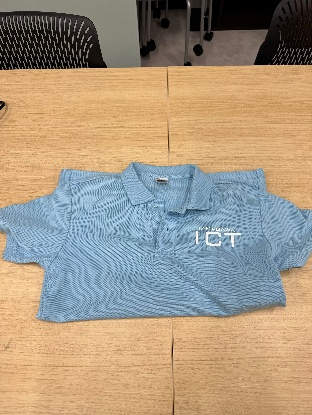
\includegraphics[height=4.5cm]{images/score-folding/image4.jpeg}}
    \hfill
    \subfloat{
        
\includegraphics[height=4.5cm]{images/score-folding/image5.jpeg}}
    \hfill
    \subfloat{
        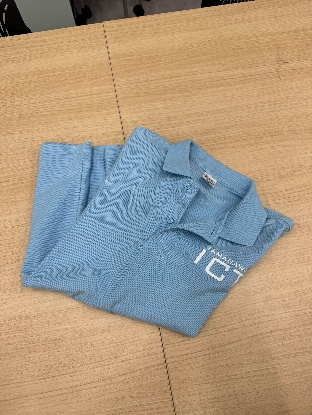
\includegraphics[height=4.5cm]{images/score-folding/image6.jpeg}}
    \caption{Left --- Example (partial success): \textbf{300 pts} --- The shirt is folded but shows misalignment or slight bunching; neater than the 250 pt example. Center --- Example (moderate success): \textbf{400 pts} --- The shirt is folded using a basic technique; the result is acceptable but less precise than higher-scoring examples. Right --- Example (good): \textbf{600 pts} --- The shirt is well folded with only minor neatness issues; edges are mostly aligned.}
\end{figure}

\begin{figure}[H]
    \centering
    \subfloat{
        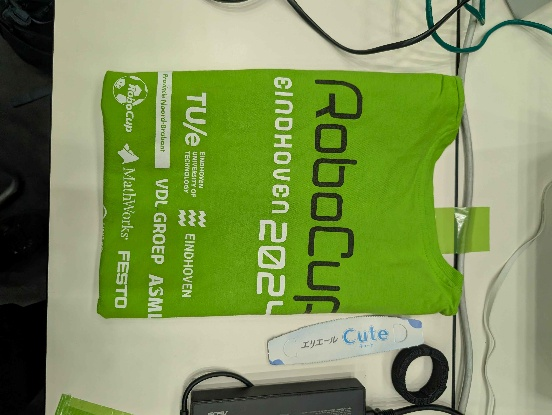
\includegraphics[height=4.5cm]{images/score-folding/image7.jpeg}}
    \hfill
    \subfloat{
        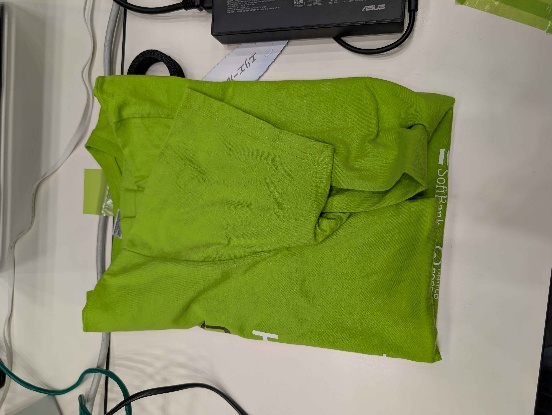
\includegraphics[height=4.5cm]{images/score-folding/image8.jpeg}}
    \caption{Example (partial success): \textbf{700 pts} --- The shirt appears folded from the front, but the back shows unintended folds where fabric is bending on top of itself outside the intended fold lines}
\end{figure}

\begin{figure}[H]
    \centering
    
\includegraphics[height=4.5cm]{images/score-folding/image10.jpeg}
    \caption{Example (success): \textbf{800 pts} --- Neatly folded}
\end{figure}

%\begin{figure}[H]
%    \centering
%    \subfloat{
%        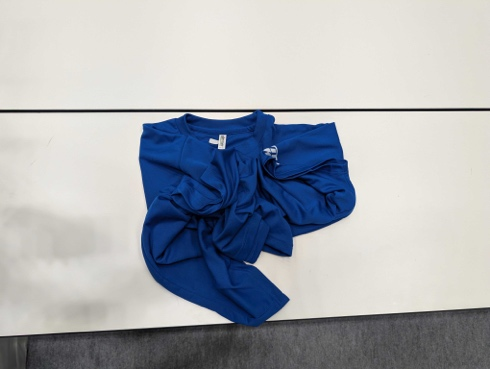
\includegraphics[height=4.5cm]{images/score-folding/image11.jpeg}}
%    \hfill
%    \subfloat{
%        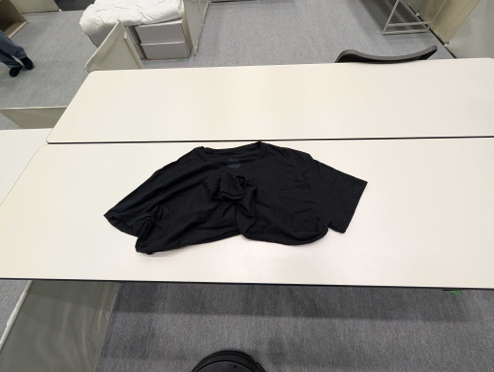
\includegraphics[height=4.5cm]{images/score-folding/image12.jpeg}}
%    \caption{Example from Japan Open}
%\end{figure}
